% FADO --- CISUC template, Beamer version.
% Compiles with pdfLaTeX, XeLaTeX, or LuaLaTeX (run twice for the TikZ overlays).
\documentclass[aspectratio=169]{beamer}
\usepackage{geometry}
\geometry{paperwidth=13.333in,paperheight=7.5in}
\usepackage{iftex}
\usepackage{tikz}
\usetikzlibrary{arrows.meta}
\usepackage{booktabs}
\usepackage{multirow}
\usepackage{amsmath}
\usepackage{array}

% ---- fonts (engine-agnostic; TeXLive-bundled Helvetica/Courier clones, no fontspec) ----
\ifPDFTeX\usepackage[utf8]{inputenc}\fi
\usepackage[T1]{fontenc}
\usepackage{textcomp}
\usepackage{tgheros}   % Helvetica clone (Arial-like) sans
\usepackage{tgcursor}  % Courier clone mono
\renewcommand{\familydefault}{\sfdefault}
\newcommand{\monofont}{\ttfamily}

% ---- colours ----
\definecolor{cred}{HTML}{DA0725}
\definecolor{ink}{HTML}{141414}
\definecolor{body}{HTML}{262626}
\definecolor{grey}{HTML}{9A9A9A}
\definecolor{lgrey}{HTML}{C4C4C4}
\definecolor{rulec}{HTML}{2A2A2A}
\definecolor{green}{HTML}{2E9E5B}
\definecolor{amber}{HTML}{C77A18}

\setbeamercolor{normal text}{fg=body}
\setbeamertemplate{navigation symbols}{}
\setbeamersize{text margin left=0pt,text margin right=0pt}

% ---- running header (shown on non-plain frames) ----
\newcommand{\hdrsec}{}
\newcommand{\hdrpg}{}
\newcommand{\pageset}[2]{\renewcommand{\hdrsec}{#1}\renewcommand{\hdrpg}{#2}}
\setbeamertemplate{headline}{%
  \vskip3mm%
  \makebox[\paperwidth][c]{%
    \hspace{9mm}%
    \parbox[t]{4.2in}{\monofont\color{grey}\fontsize{9}{11}\selectfont
      FADO: A Reaction Controller for Fairness-\\ Aware Online Learning Under Concept Drift}%
    \hfill
    \parbox[t]{4.2in}{\centering\monofont\color{grey}\fontsize{10}{12}\selectfont \hdrsec}%
    \hfill
    \parbox[t]{2.6in}{\raggedleft\monofont\fontsize{13}{15}\selectfont
      \textbf{\color{ink}\hdrpg}{\color{grey}/21}}%
    \hspace{9mm}%
  }%
}
\setbeamertemplate{footline}{}
\setbeamertemplate{frametitle}{}

% ---- helpers (absolute placement via TikZ overlay) ----
% \tb{width-in}{x-in}{y-in}{content}  --- anchored top-left at (x,y) from page NW
% optional #1 = extra node options (use font=... for large text so spacing scales)
\newcommand{\tb}[5][]{\begin{tikzpicture}[remember picture,overlay]%
  \node[anchor=north west,inner sep=0pt,outer sep=0pt,text width=#2in,align=left,#1]
    at ([xshift=#3in,yshift=-#4in]current page.north west){\raggedright #5\par};\end{tikzpicture}}
\newcommand{\fs}[2]{\fontsize{#1}{#2}\selectfont}
\newcommand{\hrl}[3]{\tb{#3}{#1}{#2}{{\color{lgrey}\rule{#3in}{0.9pt}}}}
\newcommand{\hrld}[3]{\tb{#3}{#1}{#2}{{\color{rulec}\rule{#3in}{1.3pt}}}}
% square outline cell with centred label: \boxcell{x}{y}{size-in}{label}
\newcommand{\boxcell}[4]{\begin{tikzpicture}[remember picture,overlay]%
  \node[draw=lgrey,line width=0.8pt,anchor=north west,minimum width=#3in,minimum height=#3in,
    align=center,text=ink,font=\fontsize{14}{16}\selectfont]
    at ([xshift=#1in,yshift=-#2in]current page.north west){#4};\end{tikzpicture}}
% arrow from (x1,y1) to (x2,y2) in inches from page NW
\newcommand{\parrow}[4]{\begin{tikzpicture}[remember picture,overlay]%
  \draw[-{Latex[length=2mm]},line width=1.3pt,ink]
    ([xshift=#1in,yshift=-#2in]current page.north west)--([xshift=#3in,yshift=-#4in]current page.north west);\end{tikzpicture}}
% content title at (0.85, y) --- size via node font option so spacing scales
\newcommand{\ctitle}[2][28]{\tb[font=\fontsize{#1}{#1}\selectfont\bfseries]{11.6}{0.85}{1.4}{\color{ink}#2}}
% divider
\newcommand{\divider}[2]{\tb[font=\fontsize{40}{46}\selectfont\bfseries]{11.3}{1.0}{3.05}{%
  \centering{\color{cred}#1.\ }{\color{ink}#2}}}
% column helpers (fixed y per slide type) --- defined once, avoid in-frame defs
\newcommand{\colblk}[4]{%
  \tb{3.5}{#1}{2.45}{\bfseries\color{ink}\fs{17}{20}#2}%
  \tb{3.5}{#1}{2.9}{\itshape\color{grey}\fs{12}{14}#3}%
  \hrl{#1}{3.32}{3.3}%
  \tb{3.3}{#1}{3.5}{\color{body}\fs{13.5}{17}#4}}
\newcommand{\phaseblk}[4]{%
  \tb{3.5}{#1}{2.5}{\bfseries\color{cred}\fs{17}{20}#2}%
  \tb{3.5}{#1}{2.95}{\itshape\color{grey}\fs{13}{15}#3}%
  \hrl{#1}{3.35}{3.1}%
  \tb{3.2}{#1}{3.5}{\color{body}\fs{13}{16}#4}}
\newcommand{\dcolblk}[3]{%
  \tb{3.6}{#1}{2.55}{\bfseries\color{ink}\fs{16}{19}#2}%
  \hrl{#1}{3.35}{3.3}%
  \tb{3.4}{#1}{3.5}{\color{body}\fs{14}{18}#3}}

\begin{document}

% ===================================================== 1 LOGO
\begin{frame}[plain]
  \tb{4.6}{4.37}{3.35}{
\includegraphics[width=4.6in]{assets/cisuc_logo.png}}
\end{frame}

% ===================================================== 2 TITLE
\begin{frame}[plain]
  \tb[font=\fontsize{46}{50}\selectfont\bfseries]{11.4}{0.9}{2.4}{\color{ink}FADO}
  \tb[font=\fontsize{30}{36}\selectfont\bfseries]{11.4}{0.9}{3.4}{\color{ink}A Reaction Controller for Fairness-Aware\\ Online Learning Under Concept Drift}
  \tb{11}{0.92}{4.55}{\color{ink}\fs{19}{22}Tiago Silva}
  \tb{11}{0.92}{5.35}{\color{ink}\fs{14}{18}\textbf{CISUC \textperiodcentered{} Data-Centric AI Lab}\\
    {\color{body}\fs{14}{18}Department of Informatics Engineering, University of Coimbra}}
  \tb{2.5}{0.9}{6.75}{
\includegraphics[width=2.5in]{assets/cisuc_logo.png}}
\end{frame}

% ===================================================== 3 OUTLINE (01)
\pageset{Outline}{01}
\begin{frame}
  \tb{6}{0.85}{1.55}{\bfseries\color{ink}\fs{30}{34}Outline}
  \tb[font=\fontsize{20}{34}\selectfont]{9}{2.1}{2.55}{\color{ink}\setlength{\parskip}{7pt}
    {\color{cred}\bfseries 1.}~~Motivation \& Problem\par
    {\color{cred}\bfseries 2.}~~FADO: Base Learner\par
    {\color{cred}\bfseries 3.}~~The Reaction Controller\par
    {\color{cred}\bfseries 4.}~~Experimental Design\par
    {\color{cred}\bfseries 5.}~~Results\par
    {\color{cred}\bfseries 6.}~~Intersectional Fairness\par
    {\color{cred}\bfseries 7.}~~Takeaways \& Next Steps}
\end{frame}

% ===================================================== S1 divider (02)
\begin{frame}[plain]\divider{1}{Motivation \& Problem}\end{frame}

% ---- 1.1 (03) ----
\pageset{1.Motivation \& Problem}{03}
\begin{frame}
  \ctitle{Concept drift degrades {\color{cred}\underline{fairness}}, not only accuracy}
  \tb{7.1}{0.85}{2.5}{\color{body}\fs{17}{23}\setlength{\parskip}{9pt}
    Fairness-aware learners are trained assuming a \textbf{stationary} distribution.\par
    Real streams \textbf{\underline{drift}}: P(y\,$\vert$\,x) and base rates move with policy, behavioural and economic change.\par
    Drift breaks the statistical relationships fairness rests on --- so \textbf{bias can grow while accuracy looks stable}.}
  \hrl{8.35}{2.6}{4.1}
  \tb{4.1}{8.35}{2.75}{\fs{14}{18}{\color{cred}\bfseries RQ1}\\[2pt]
    {\color{ink}To what extent does drift affect group-fairness metrics online?}}
  \hrl{8.35}{4.35}{4.1}
  \tb{4.1}{8.35}{4.5}{\fs{14.5}{18}{\color{cred}\bfseries RQ2}\\[2pt]
    {\color{ink}Can adaptive detection \& response preserve fairness while keeping performance?}}
\end{frame}

% ---- 1.2 (04) ----
\pageset{1.Motivation \& Problem}{04}
\begin{frame}
  \ctitle{Keep the in-processing fairness; add the drift machinery}
  \colblk{0.85}{In-processing fair}{e.g. Aranyani, RFR}{Fair during training\\[3pt]No drift detection\\[3pt]Regulariser is static}
  \colblk{4.85}{Drift-adaptive}{e.g. ARF}{Detect \& react to shift\\[3pt]Accuracy-driven only\\[3pt]No fairness mechanism}
  \colblk{8.85}{Drift-aware fair}{prior attempts}{Shift as fixed perturbation\\[3pt]Worst-case, not streaming\\[3pt]No online controller}
  \parrow{6.66}{5.72}{6.66}{6.12}
  \tb{11.6}{0.85}{6.28}{\centering\fs{15}{19}{\color{cred}\bfseries\fs{20}{20}FADO}\ \ {\color{ink}= retain Aranyani's node-level fairness regulariser, then wrap it in an online detector + reaction controller.}}
  \tb{11.6}{0.85}{6.95}{\centering\itshape\color{grey}\fs{12}{14}Aranyani is inherited, not contributed --- the novelty is the drift-detection-and-response layer.}
\end{frame}

% ===================================================== S2 divider (05)
\begin{frame}[plain]\divider{2}{FADO: Base Learner}\end{frame}

% ---- 2.1 (06) ----
\pageset{2.FADO: Base Learner}{06}
\begin{frame}
  \ctitle{Why a {\color{cred}soft-routed oblique} forest}
  \tb{11.6}{0.85}{2.4}{\color{body}\fs{16.5}{22}\setlength{\parskip}{8pt}
    \textbf{\underline{Oblique}} nodes split on a \textbf{linear combination of features} (an angled hyperplane) --- far more expressive per node than axis-aligned splits.\par
    A temperature-scaled \textbf{sigmoid} makes routing soft and differentiable, so the whole forest trains by gradient descent, online --- and each node acts as a per-step prediction, letting fairness be imposed at \textbf{\underline{every node}}.}
  \hrl{3.3}{4.75}{6.7}
  \tb{11.6}{0.85}{4.95}{\centering\fs{22}{26}$\displaystyle n_j(x)=\sigma\!\left((w_j^{\top}x + b_j)\,/\,{\color{cred}\tau}\right)\in(0,1)$}
  \tb{11.6}{0.85}{5.85}{\centering\fs{21}{25}$\displaystyle f(x)=\tfrac{1}{K}\textstyle\sum_k \mathrm{softmax}\!\left(f_k(x)\right)$}
  \tb{11.6}{0.85}{6.75}{\centering\color{body}\fs{13.5}{17}Parameter isolation $\to$ cheap per-step gradient \textperiodcentered{} O(W) streaming memory \textperiodcentered{} {\color{cred}\bfseries temperature $\tau$ is the controller's lever} ($\tau$=1 smooth learning; $\tau\to$0 decisive recovery).}
\end{frame}

% ---- 2.2 (07) : trained oblique-tree demonstration ----
\pageset{2.FADO: Base Learner}{07}
\begin{frame}
  \ctitle{Oblique + soft routing, learned by {\color{cred}backpropagation}}
  \tb{8.5}{2.42}{2.0}{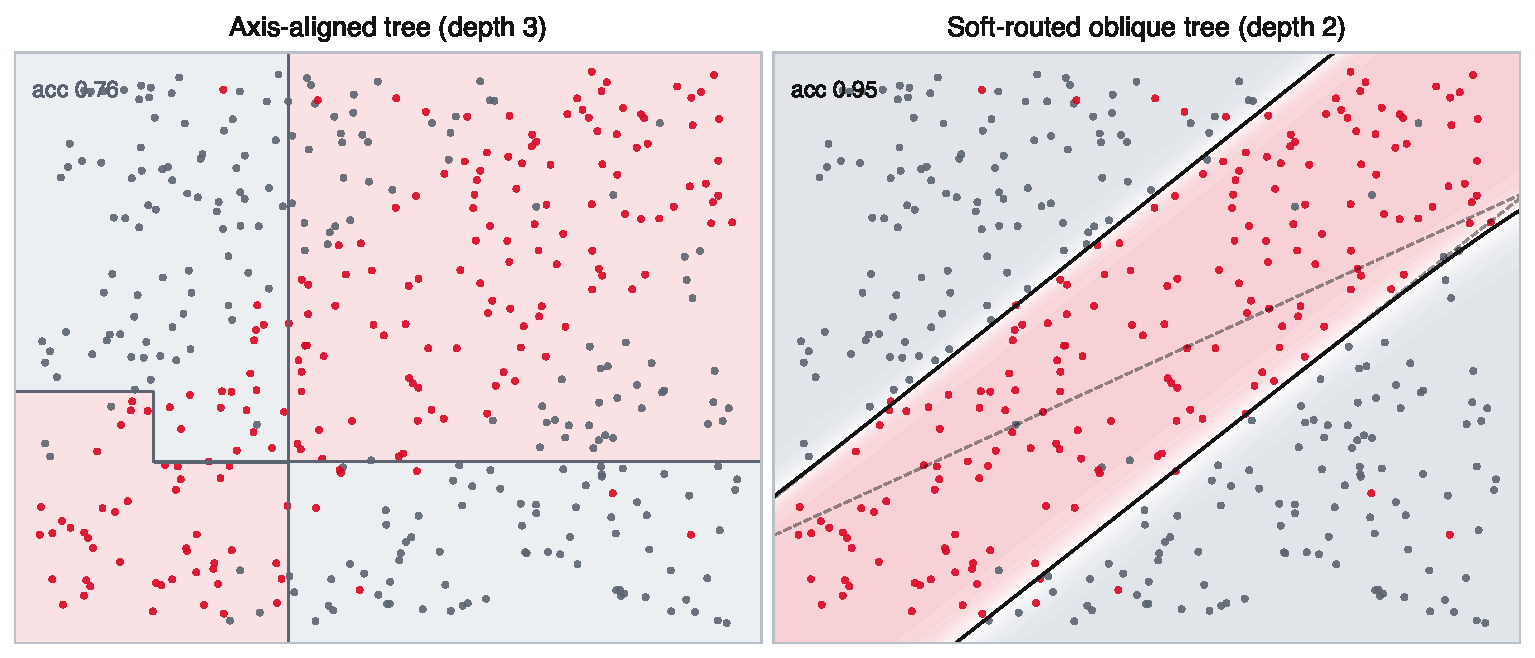
\includegraphics[width=8.5in]{assets/oblique_demo.pdf}}
  \tb{11.6}{0.85}{5.62}{\centering\color{body}\fs{13}{16}Same diagonal-stripe data: axis-parallel splits approximate it with a \textbf{staircase}; two \textbf{oblique} hyperplanes capture the band, and the shading is the \textbf{soft} routing probability. \emph{(A depth-2 soft oblique tree, trained here by gradient descent.)}}
  \hrl{3.3}{6.18}{6.7}
  \tb{11.6}{0.85}{6.38}{\centering\fs{17}{21}$\displaystyle p(x)=\sum_{\ell}P_\ell(x)\,s_\ell,\quad P_\ell(x)=\!\!\prod_{j\in\mathrm{path}(\ell)}\!\! g_j\,\text{or}\,(1{-}g_j),\quad g_j=\sigma(w_j^{\top}x+b_j)$}
  \tb{11.6}{0.85}{7.02}{\centering\color{body}\fs{12.5}{15}Every gate is a differentiable sigmoid, so $p(x)$ is smooth in every weight --- \textbf{trainable by backpropagation, one sample at a time}; the same gates $g_j$ carry the fairness penalty and the temperature $\tau$.}
\end{frame}

% ---- 2.3 (08) : regulariser ----
\pageset{2.FADO: Base Learner}{08}
\begin{frame}
  \ctitle{A per-node DP gap, smoothed by a {\color{cred}Huber surrogate}}
  \tb{11.6}{0.85}{2.35}{\color{body}\fs{16.5}{22}At each routing node, compare the group-conditional mean routing to the cross-group mean --- the per-node analogue of the demographic-parity gap --- and sum the penalty over \textbf{every node in every tree}.}
  \hrl{3.3}{3.95}{6.7}
  \tb{11.6}{0.85}{4.28}{\centering\fs{22}{26}$\displaystyle F_{\color{cred}a}=\bar{n}-\bar{n}_{\color{cred}a}$}
  \tb{11.6}{0.85}{5.08}{\centering\fs{21}{25}$\displaystyle \mathcal{L}=\mathcal{L}_{\mathrm{CE}}+\lambda\textstyle\sum_{\mathrm{nodes}}\tfrac{1}{K}\sum_a \phi_\delta(F_a)$}
  \tb{11.6}{0.85}{5.88}{\centering\fs{19}{23}$\displaystyle \phi_\delta'(z)=z\ \text{if}\ |z|<\delta,\quad \mathrm{sign}(z)\ \text{if}\ |z|\ge\delta$}
  \tb{11.6}{0.85}{6.55}{\centering\color{body}\fs{13.5}{17}Quadratic near 0 (smooth gradient) \textperiodcentered{} linear tail (bounded outlier influence) \textperiodcentered{} \textbf{unit-slope tail $\to$ firmer correction past $\delta$}. DP defined as deviation-from-mean to match the regulariser exactly.}
\end{frame}

% ===================================================== S3 divider (09)
\begin{frame}[plain]\divider{3}{The Reaction Controller}\end{frame}

% ---- 3.1 (10) ----
\pageset{3.The Reaction Controller}{10}
\begin{frame}
  \ctitle{Two detectors, three phases, one {\color{cred}temperature}}
  \phaseblk{0.85}{WARN}{pre-warm}{Sensitive $D_w$ trips\\[3pt]LR $\times\,\beta_w$ (=5)\\[3pt]arm --- don't commit}
  \phaseblk{4.9}{CONFIRM}{spike + sharpen}{Strict $D_c$ confirms\\[3pt]LR $\times\,\beta_c$ (=10)\\[3pt]$\tau\to\tau_{\mathrm{drift}}$=0.1\\[3pt]reset detectors}
  \phaseblk{8.95}{RECOVER}{anneal back}{$\eta\to\eta_0$ over $\Delta$\\[3pt]$\tau\to$1\\[3pt]cooldown C=200}
  \parrow{4.4}{3.05}{4.85}{3.05}
  \parrow{8.45}{3.05}{8.9}{3.05}
  \hrl{3.3}{5.5}{6.7}
  \tb{11.6}{0.85}{5.85}{\centering\fs{20}{24}$\displaystyle \varepsilon_{\color{cred}\mathrm{cut}}=\sqrt{\tfrac{1}{2m}\,\ln\tfrac{4}{\delta}}$}
  \tb{11.6}{0.85}{6.6}{\centering\fs{13.5}{17}{\color{ink}\bfseries $\delta$ calibrated to stream length ($\varepsilon\propto 1/\sqrt{m}$).}\ {\color{body}Label-noise guard ($\nu$=0.7) excludes confident-but-wrong points, so noise can't fire the controller.}}
\end{frame}

% ---- 3.2 (11) ----
\pageset{3.The Reaction Controller}{11}
\begin{frame}
  \ctitle{The prequential loop}
  \tb{10.4}{1.47}{2.15}{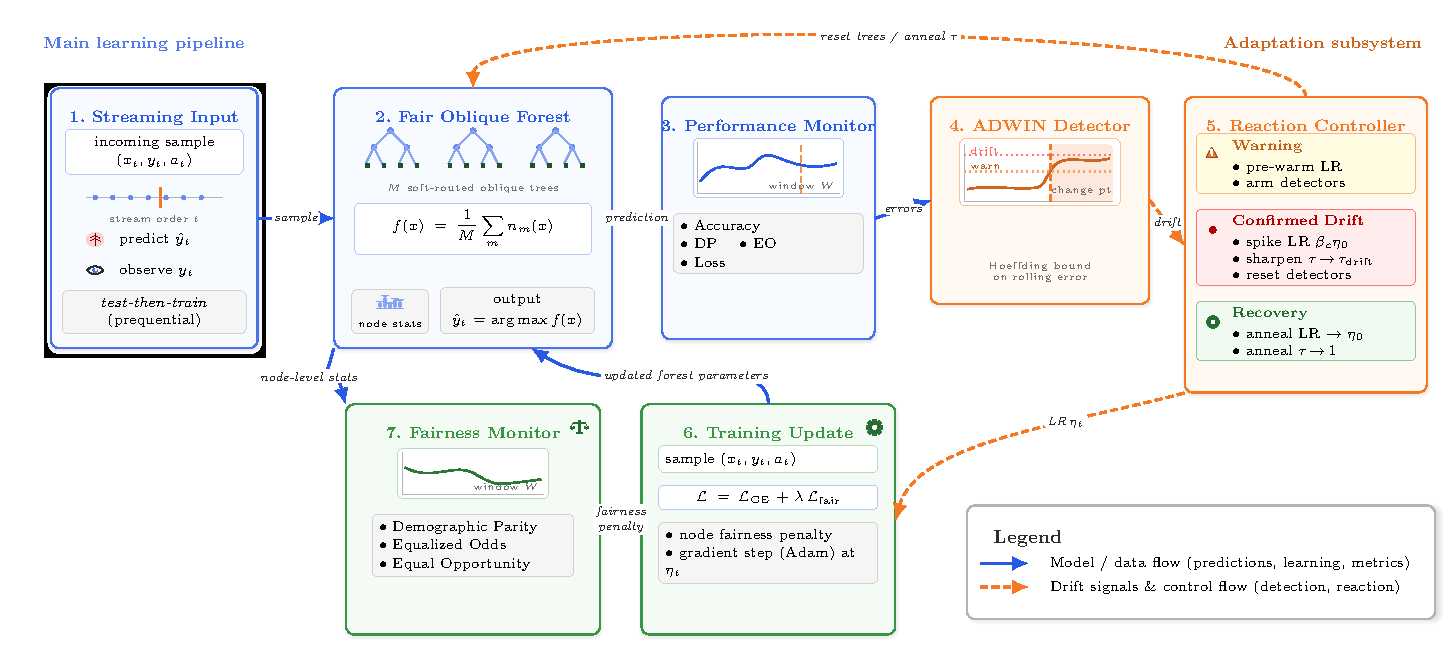
\includegraphics[width=10.4in]{assets/fado_figure.pdf}}
  \tb{11.6}{0.85}{6.85}{\centering\color{grey}\fs{12.5}{15}Blue = data flow through the fair forest.\quad Orange = drift signals \& control flow: detector $\to$ controller $\to$ retuned gradient step.}
\end{frame}

% ===================================================== S4 divider (12)
\begin{frame}[plain]\divider{4}{Experimental Design}\end{frame}

% ---- 4.1 (13) ----
\pageset{4.Experimental Design}{13}
\begin{frame}
  \ctitle{Two complementary {\color{cred}drift regimes}}
  \dcolblk{0.85}{Folktables --- natural, gradual}{ACS Income (CA), \textasciitilde187k rows\\[5pt]Real cross-year shift\\[5pt]2015 train $\to$ 2017--18 stream\\[5pt]Group = sex $\times$ race (joint)}
  \dcolblk{4.85}{COMPAS --- synthetic, abrupt}{7.2k rows, controlled testbed\\[5pt]Symmetric race swap +\\[5pt]Bernoulli(0.5) label flip\\[5pt]no\_drift vs abrupt\_race}
  \dcolblk{8.85}{Protocol}{Prequential test-then-train\\[5pt]Batch 1 \textperiodcentered{} 30 pinned seeds\\[5pt]Paired Wilcoxon + Holm\\[5pt]Welch t-test cross-check}
  \tb{11.6}{0.85}{6.4}{\fs{13.5}{17}{\color{ink}\bfseries Baselines (held fixed):} {\color{body}ARF (adaptive, unfair), RFR (fair, static), and a controller-free Aranyani ablation sharing learner, loss, window and seed-pinned data order --- so any FADO--Aranyani gap is the controller alone.}}
\end{frame}

% ===================================================== S5 divider (14)
\begin{frame}[plain]\divider{5}{Results}\end{frame}

% ---- 5.1 marginal, DP only (15) ----
\pageset{5.Results}{15}
\begin{frame}
  \ctitle[24]{Marginal DP --- drift erodes fairness; controller helps on {\color{cred}abrupt} shift}
  \tb{6.0}{0.85}{2.5}{\color{ink}\fs{13}{16}%
    \renewcommand{\arraystretch}{1.45}%
    \begin{tabular}{@{}l l r r@{}}
    \toprule
    \textbf{Dataset} & \textbf{Model} & \textbf{Acc}\,$\uparrow$ & \textbf{DP}\,$\downarrow$\\
    \midrule
    \multirow{4}{*}{\textbf{Folktables}}
      & {\color{cred}\textbf{FADO}} & {\color{cred}0.8033} & {\color{cred}\textbf{0.0284}\textsuperscript{**}}\\
      & Aranyani & \textbf{0.8053} & 0.0299\\
      & ARF & 0.7447 & 0.0722\\
      & RFR & 0.7780 & 0.0733\\
    \midrule
    \multirow{4}{*}{\textbf{COMPAS}}
      & {\color{cred}\textbf{FADO}} & {\color{cred}0.6434} & {\color{cred}\textbf{0.0611}\textsuperscript{***}}\\
      & Aranyani & \textbf{0.6451} & 0.0679\\
      & ARF & 0.6313 & 0.0808\\
      & RFR & 0.6404 & 0.0813\\
    \bottomrule
    \end{tabular}}
  \tb{5.0}{7.4}{2.5}{\bfseries\color{ink}\fs{14}{17}Reading the table}
  \tb{5.0}{7.4}{3.0}{\fs{13.5}{17}\setlength{\parskip}{9pt}
    {\color{cred}\bfseries RQ1.} {\color{body}Both external baselines carry \textasciitilde2$\times$ FADO's DP on both regimes (all p$<$0.001).}\par
    {\color{cred}\bfseries Regime-dependent.} {\color{body}On abrupt COMPAS the controller cuts DP by 0.68pp (p$<$0.001).}\par
    {\color{body}\textbf{On gradual Folktables} it ties the base learner --- a smooth shift needs no spike.}}
  \tb{6.0}{0.85}{6.75}{\itshape\color{grey}\fs{10.5}{13}Bold = best per metric within dataset;\ \ ** p$<$0.01, *** p$<$0.001 (paired Wilcoxon, Holm) vs every baseline.}
\end{frame}

% ===================================================== S6 divider (16)
\begin{frame}[plain]\divider{6}{Intersectional Fairness}\end{frame}

% ---- 6.1 gameable / composite (17) ----
\pageset{6.Intersectional Fairness}{17}
\begin{frame}
  \ctitle{Marginal parity is {\color{cred}provably gameable}}
  \tb{7.0}{0.85}{2.4}{\color{body}\fs{16.5}{22}\setlength{\parskip}{9pt}
    Enforcing parity on \textbf{each attribute separately} is defeatable (Kearns et al., 2018): a model can be perfectly fair on sex \textit{and} on race, yet badly unfair on a \textbf{\underline{joint}} subgroup --- fairness gerrymandering.\par
    FADO optimises parity over the \textbf{Cartesian-product subgroups}. The regulariser already supports arbitrary K\,$\ge$\,2 --- the learner needed no change.}
  \hrl{0.85}{5.15}{6.7}
  \tb{6.7}{0.85}{5.4}{\centering\fs{23}{27}$\displaystyle a=2a_{\color{cred}1}+a_{\color{cred}2}\ \in\ \{0,1,2,3\}$}
  \tb{6.7}{0.85}{6.35}{\itshape\color{grey}\fs{12.5}{15}One 4-valued composite index replaces two binary axes.}
  \tb{3.95}{8.5}{2.2}{\centering\bfseries\color{ink}\fs{14}{16}Four joint cells}
  \boxcell{8.5}{2.7}{1.85}{$a_1$=0, $a_2$=0}
  \boxcell{10.6}{2.7}{1.85}{$a_1$=0, $a_2$=1}
  \boxcell{8.5}{4.75}{1.85}{$a_1$=1, $a_2$=0}
  \boxcell{10.6}{4.75}{1.85}{$a_1$=1, $a_2$=1}
\end{frame}

% ---- 6.2 intersectional results (18) ----
\pageset{6.Intersectional Fairness}{18}
\begin{frame}
  \ctitle[24]{Intersectional grouping surfaces the {\color{cred}controller's contribution}}
  \tb{7.2}{0.85}{2.55}{\color{ink}\fs{12.5}{15}%
    \renewcommand{\arraystretch}{1.5}%
    \begin{tabular}{@{}l r r r r@{}}
    \toprule
    \textbf{Model} & \textbf{Acc}\,$\uparrow$ & \textbf{DP}\,$\downarrow$ & \textbf{DP sex}\,$\downarrow$ & \textbf{DP race}\,$\downarrow$\\
    \midrule
    {\color{cred}\textbf{FADO}} & {\color{cred}0.7979} & {\color{cred}\textbf{0.0688}} & {\color{cred}\textbf{0.0234}} & {\color{cred}\textbf{0.0243}}\\
    Aranyani & \textbf{0.8005} & 0.0727 & 0.0283 & 0.0294\\
    ARF & 0.7446 & 0.1497 & 0.0735 & 0.0620\\
    RFR & 0.7779 & 0.1427 & 0.0724 & 0.0591\\
    \bottomrule
    \end{tabular}}
  \tb{7.2}{0.85}{4.75}{\itshape\color{grey}\fs{10.5}{13}DP = joint violation over the four cells (optimised);\ \ DP sex / DP race = marginal diagnostics.\ \ Bold = best mean.}
  \tb{4.15}{8.35}{2.6}{\bfseries\color{cred}\fs{14}{17}The controller now measurably wins}
  \tb{4.15}{8.35}{3.1}{\color{body}\fs{13.5}{17}vs the controller-free forest: DP $-$0.38pp, significant under \textbf{both} Wilcoxon (p$<$0.001) and Welch (p$<$0.01) --- where the marginal view was only a tie.}
  \tb{4.15}{8.35}{4.95}{\bfseries\color{cred}\fs{14}{17}Gerrymandering, confirmed}
  \tb{4.15}{8.35}{5.45}{\color{body}\fs{13.5}{17}Intersectional-to-worst-marginal DP ratio $\approx$ 2.8 (FADO), 2.5 (Aranyani), \textasciitilde2.0 (ARF/RFR): the fairest learners hide the largest joint gap.}
\end{frame}

% ===================================================== S7 divider (19)
\begin{frame}[plain]\divider{7}{Takeaways \& Next Steps}\end{frame}

% ---- 7.1 (20) ----
\pageset{7.Takeaways \& Next Steps}{20}
\begin{frame}
  \ctitle{What we learned --- and what's next}
  \tb{7.0}{0.85}{2.4}{\bfseries\color{cred}\fs{16}{19}Takeaways}
  \tb{7.0}{0.85}{2.9}{\color{body}\fs{15}{19}\setlength{\parskip}{9pt}
    \textbf{RQ1.} Drift is a fairness problem --- it inflates the DP of accuracy-only and static-fair baselines alike.\par
    \textbf{RQ2.} An adaptive fair learner keeps both utility and fairness; the controller earns its keep on abrupt shift.\par
    \textbf{Design.} The fairness objective must match the harm: node-level DP + a joint group index makes the penalty cheap and the controller's gain measurable.}
  \tb{4.15}{8.35}{2.4}{\bfseries\color{cred}\fs{16}{19}Next}
  \tb{4.15}{8.35}{2.9}{\color{body}\fs{15}{19}\setlength{\parskip}{9pt}
    \textbf{\underline{Controller ablation}} --- isolate each phase; the most targetable point.\par
    \textbf{Optimise EO directly} (wire the existing EO regulariser into the gradient).\par
    \textbf{Finish the COMPAS intersectional sweep} and re-verify gerrymandering.}
\end{frame}

% ===================================================== CLOSING (21)
\begin{frame}[plain]
  \tb[font=\fontsize{40}{46}\selectfont\bfseries]{11.5}{0.9}{2.7}{\color{ink}Fairness that adapts}
  \tb{11.4}{0.92}{3.85}{\fs{19}{24}{\color{body}A drift-aware controller keeps an intersectionally-fair oblique forest fair }{\color{cred}\bfseries as the distribution moves.}}
  \tb{11.4}{0.92}{5.2}{\bfseries\color{ink}\fs{18}{22}Thank you --- questions \& discussion}
  \tb{11.4}{0.92}{5.7}{\color{grey}\fs{13}{16}Tiago Silva \textperiodcentered{} CISUC Data-Centric AI Lab \textperiodcentered{} FADO (submitted to ICDM 2026)}
  \tb{2.2}{0.9}{6.7}{
\includegraphics[width=2.2in]{assets/cisuc_logo.png}}
\end{frame}

% ===================================================== BACKUP 1: interpretability
\begin{frame}[plain]
  \tb{6}{0.85}{0.5}{\monofont\color{grey}\fs{11}{13}BACKUP \textperiodcentered{} interpretability}
  \ctitle{Is a forest more interpretable than a DNN?}
  \tb{11.7}{0.85}{2.45}{\color{ink}\fs{14}{17}%
    \renewcommand{\arraystretch}{1.7}%
    \begin{tabular}{@{}p{4.9in} c c c@{}}
    \toprule
    \textbf{Sense of ``interpretable''} & \textbf{Axis-aligned tree} & \textbf{Soft oblique forest} & \textbf{Deep NN}\\
    \midrule
    \textbf{Simulatability} {\color{grey}\fs{12}{12}-- trace one prediction} & {\color{green}\bfseries Yes} & {\color{amber}\bfseries Partial} & {\color{cred}\bfseries No}\\
    \textbf{Decomposability} {\color{grey}\fs{12}{12}-- parts carry meaning} & {\color{green}\bfseries Yes} & {\color{green}\bfseries Yes} & {\color{cred}\bfseries No}\\
    \textbf{Post-hoc} {\color{grey}\fs{12}{12}-- SHAP / saliency} & {\color{green}\bfseries Yes} & {\color{green}\bfseries Yes} & {\color{green}\bfseries Yes}\\
    \bottomrule
    \end{tabular}}
  \hrl{0.85}{5.35}{11.6}
  \tb{11.6}{0.85}{5.55}{\color{body}\fs{14.5}{19}\setlength{\parskip}{7pt}
    \textbf{Oblique} (linear-combination splits) and \textbf{soft} routing (probabilistic paths) trade rule-level transparency for expressiveness + differentiability --- so it is \emph{not} as readable as a plain if-then tree.\par
    {\color{cred}\bfseries What FADO actually leans on is decomposability:} fairness is enforced and audited \textbf{per routing node} --- a structure a monolithic network simply does not have.}
\end{frame}

% ===================================================== BACKUP 2: why backprop
\begin{frame}[plain]
  \tb{6}{0.85}{0.5}{\monofont\color{grey}\fs{11}{13}BACKUP \textperiodcentered{} why backpropagation}
  \ctitle{Why backpropagation is the {\color{cred}enabling mechanism}}
  \tb{11.7}{0.85}{2.35}{\color{body}\fs{14}{18}Reverse-mode autodiff: gradients w.r.t.\ \textbf{all} parameters in one backward pass, at $\sim$the cost of one forward pass (finite differences would cost one pass \emph{per} parameter).}
  \hrl{0.85}{3.25}{11.6}
  \tb{11.7}{0.85}{3.45}{\color{body}\fs{14.5}{20}\setlength{\parskip}{8pt}
    {\color{cred}\bfseries 1.\ Makes ``soft'' pay off.}\ Train all oblique hyperplanes \emph{jointly} by gradient descent, instead of greedy CART splits.\par
    {\color{cred}\bfseries 2.\ Enables streaming.}\ Cheap per-sample SGD step --- the model adapts incrementally as the stream flows; a greedy tree cannot update per sample.\par
    {\color{cred}\bfseries 3.\ Lets fairness enter training.}\ $\mathcal{L}=\mathcal{L}_{\mathrm{CE}}+\lambda\,\mathcal{L}_{\mathrm{fair}}$: backprop carries \emph{both} the accuracy and the fairness gradient to every node.\par
    {\color{cred}\bfseries 4.\ The controller needs a gradient loop.}\ It modulates the learning rate $\eta$ and temperature $\tau$ --- knobs that only exist under gradient training.\par
    {\color{cred}\bfseries 5.\ Keeps the step cheap.}\ Node-local fairness $\Rightarrow$ the fairness gradient is O(nodes), fast enough for real-time streams.}
\end{frame}

\end{document}
